\subsection{Sviluppi futuri}
Sebbene il pacchetto Python sia funzionante, testato e documentato, non si può dire che sia pienamente applicabile ad un gran numero di problemi pratici. Può essere utilizzato senza dubbio per la riduzione di grafi, ma vi sono alcune funzionalità critiche nella pratica che al momento non sono ancora implementate. Ne elenchiamo brevemente alcune, giustificando i motivi che ci portano a considerarne l'integrazione:
\begin{itemize}
    \item \emph{Labeled edges}: come abbiamo osservato nella Sezione \ref{sec:applitations} assegnare etichette agli archi consente di modellizzare problemi molto complessi ed interessanti, dunque integrare questa funzionalità aumenterebbe molto l'applicabilità del pacchetto;
    \item \emph{k-bisimulazione}: in alcuni casi la bisimulazione fornisce un partizionamento del grafo troppo approfondito, inutilizzabile all'atto pratico, poichè ciò che succede ``lontano'' da un nodo talvolta è di poca importanza per quel nodo; per questo motivo si introduce una variante, la k-bisimulazione, in cui le caratteristiche topologiche di un nodo (gli archi nella sua immagine, gli archi nell'immagine dei successori del nodo, \dots) vengono considerate solo in un ``intorno'' di raggio $k \geq 0$ \cite{kbisi}; la k-bisimulazione peraltro è piuttosto economica da calcolare, e trova quindi diverse applicazioni pratiche;
    \item \emph{NetworkX}: la libreria Python \emph{NetworkX} contiene numerose funzioni utili per i grafi (come ad esempio la visità in profondità, o l'algoritmo di Kosaraju) che tuttavia si applicano unicamente ad oggetti di tipo \verb|networkx.Graph|; nelle prime fasi dello sviluppo si è deciso di non percorrere la possibilità di implementare il pacchetto rappresentando i grafi con gli oggetti forniti da \emph{NetworkX}, ma piuttosto di creare classi apposite (\emph{\_Vertex, \_Edge}, \dots) in quanto l'autore riteneva (erroneamente) che l'accesso agli attributi dell'istanza di una classe fosse $O(1)$, mentre per salvare attributi all'interno di un oggetto di \emph{NetworkX} è necessario passare per un dizionario; questa assunzione si è rivelata chiaramente falsa quando si è utilizzato lo strumento \emph{cProfile} (Figura \ref{fig:cprofile_result}), e dunque non c'è più nessun motivo per non passare, in futuro, ad un approccio puramente \emph{NetworkX}-friendly.
\end{itemize}

\begin{figure}
    \centering
    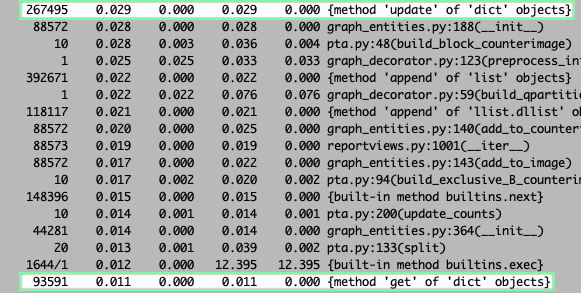
\includegraphics[width=0.7\textwidth]{./sezione3/future/resources/profiler.png}
    \caption{Output fornito da cProfile per una delle funzioni implementate nel pacchetto, sono evidenziate le righe corrispondenti ad interrogazioni o aggiornamenti di un dizionario.}
    \label{fig:cprofile_result}
\end{figure}

Intendiamo continuare lo sviluppo del pacchetto poichè riteniamo che il progetto meriti di essere sviluppato ulteriormente, e non ne abbiamo trovati altri in Python che trattino la bisimulazione in modo approfondito.
